% !TEX root = ../manuscript.tex

%%%%%%%%%%%%%%%%%%%%%%%%%%%%%%%%%%%%%%%%%%%%%%%%%%%%%%%%%%%%%%%%%%%%%
%% Start the main manuscript here.
%%%%%%%%%%%%%%%%%%%%%%%%%%%%%%%%%%%%%%%%%%%%%%%%%%%%%%%%%%%%%%%%%%%%%

\section{Introduction}

Biogas capture from landfill sites or wastewater treatment plants is identified
as an appealing strategy to procure a renewable energy fuel, simultaneously
promoting a reduction in greenhouse gas emissions and an increase in waste
treatment profitability \citep{themelisMethaneGenerationLandfills2007}. The use
of biogas as an energy green resource critically calls for a substantial
increase of its \ce{CH4} quality by removing gaseous and vapour impurities
resulting from anaerobic digestion processes
\citep{themelisMethaneGenerationLandfills2007}. One prominent class of biogas
impurities are the linear (denoted ``L'') and cyclic (denoted ``D'') siloxanes,
as degradation by-products of silicone polymers from packaging, construction,
cosmetics, and household items
\citep{takuwaCharacterizationTraceConstituents2009,
ohannessianVolatileOrganicSilicon2008}. This family of molecules is also known
to damage subsequent energy recovery systems, e.g. combustion engines, fuel
cells and steam reformers, via their decomposition into amorphous silica on
heated surfaces that leads to abrasive solid deposits on critical machinery and
to inactivation of gas reforming catalysts \citep{wangRecentAdvancesTechnologies2019}.
Octamethylcyclotetrasiloxane commonly labelled D4 is the most representative
siloxane species present in biogas, which spans from 50 to 70\% of the total
siloxane content due to its relatively low water solubility as compared to
lighter siloxanes (\SI{56}{\micro\gram\per\litre}) and its significant vapour
pressure (\SI{196}{\pascal} at \SI{30}{\degreeCelsius})
\citep{ohannessianVolatileOrganicSilicon2008,
wangRecentAdvancesTechnologies2019, dewilEnergyUseBiogas2006}.

Multiple technologies have been proposed to mitigate the presence of siloxanes
in biogas outlet streams, including mineral acid/base scrubbing, deep chilling,
or iron oxide beds, often working in tandem to remove other impurities
\citep{kuhnRequirementsTechniquesCosts2017}. The physisorption-based removal of
D4 by porous filters is also a promising alternative, due to its relatively low
potential energetic cost, while avoiding the use of environmentally hazardous
chemicals \citep{chinStatisticalAnalysisTrace2020,
ajharSiloxaneRemovalLandfill2010}. A variety of conventional adsorbents has been
envisaged for siloxane elimination, including activated carbons
\citep{finocchioDecompositionHexamethylcyclotrisiloxaneSolid2008}, zeolites
\citep{montanariPurificationLandfillBiogases2010}, and silicas
\citep{sigotAdsorptionOctamethylcyclotetrasiloxaneD42015}. However, these
materials suffer from several drawbacks that limit their commercial use, in
particular insufficient uptake and/or incomplete regeneration under standard
conditions. Moreover, downstream biogas commonly contains traces of water, which
can compete with D4 sorption when using hydrophilic adsorbents
\citep{kuhnRequirementsTechniquesCosts2017,schweigkoflerRemovalSiloxanesBiogases2001}.
Therefore, finding a high capacity adsorbent capable of removing siloxanes under
moderate humidity conditions in a reversible manner remains a challenge.

\begin{widefigure}[htb]
    \centering
    \includegraphics[width=0.95\textwidth]{ensemble_schema}
    \caption{%
        Workflow of the strategy applied to identify the best MOFs for
        D4 adsorption, narrowing down candidates from top to bottom through
        synergistic computational (left) and experimental (right) actions. The
        final MOF candidate, PCN-777, is highlighted.
    }\label{fig:overview}
\end{widefigure}

Metal-Organic Frameworks (MOFs) are one of the most recent classes of porous
adsorbents. These coordination polymers are built from the assembly of metal
nodes and organic multidentate linkers to form architectures of different
dimensionality from 1D to 4D \citep{fereyHybridPorousSolids2008,
zhouIntroductionMetalOrganic2012,
evansFourdimensionalMetalorganicFrameworks2020}. Their near-infinite diversity,
akin to a wide set of building blocks, has made this class of porous solids
ideal for applications in gas/vapor adsorption/separation
\citep{siegelmanChallengesOpportunitiesAdsorptionbased2019,
linMicroporousMetalOrganicFramework2020}, catalysis
\citep{bavykinaMetalOrganicFrameworks2020}, and sensing
\citep{allendorfElectronicDevicesUsing2020,
woellnerAdsorptionDetectionHazardous2018} among others. Their high and uniform
porosity combined with a high chemical tunability of their pore walls suggest
that MOFs may hold promise as candidates for siloxane adsorption. Insofar only
two studies have attempted to investigate the potential of MOFs for D4 removal
\citep{mito-okaSiloxaneD4Capture2013}. Mito-Oka and co-workers
\citep{mito-okaSiloxaneD4Capture2013} proposed DUT-4 (\ce{[Al(OH)(2,6-ndc)},
DUT: Dresden University of Technology), a wine rack-like MOF, as a first
potential adsorbent. Although its hydrophobicity makes this MOF attractive for
D4 elimination under humidity, its adsorption capacity of
\SI{0.15}{\gram\per\gram}, estimated as single component by TGA measurements, is
rather low and its regeneration can only be achieved at very high temperature,
over \SI{523}{\kelvin}, resulting from a high confinement of D4 (kinetic
diameter of \SI{8.6}{\angstrom}) in its channels (9 Å × 9 Å). More recently,
MIL-101(Cr) (\ce{Cr3O(OH)(H2O)2(btc)3}, MIL: Material of Institute Lavoisier), a
well-known highly porous MOF incorporating two types of mesoporous cages with
diameters of 29 Å and 34 Å was demonstrated to exhibit a record D4 uptake of
\SI{0.95}{\gram\per\gram} at \SI{298}{\kelvin}, however its regeneration was
only possible upon heating at \SI{423}{\kelvin} under vacuum
\citep{gargiuloChromiumbasedMIL101Metal2019}. Further, since MIL-101(Cr) is
known to be highly hydrophilic \citep{zhaoSynthesisMIL101Cr2020} we can expect a
substantial drop of its D4 uptake performance even under low-relative humidity.
Indeed, neither of these MOFs tested so far combines large D4 uptake, low-energy
regeneration and hydrophobicity to avoid a preferential adsorption of \ce{H2O}
over D4 under low to moderate relative humidity.

To date, only a very small number of MOFs has been sampled for this application,
and therefore relied on researchers' intuition to identify promising adsorbents.
There are, however, a myriad of hydrophobic MOFs that can potentially perform
better for D4 adsorption. Since it is unfeasible to individually test the
performances of all the existing MOFs, several high throughput computational
screening (HTCS) workflows have been devised which identified promising MOFs for
diverse for diverse adsorption-related applications \citep{simonWhatAreBest2015,
parkEstablishingUpperBounds2017, moghadamComputeraidedDiscoveryMetal2018,
boydDatadrivenDesignMetal2019, shiMachineLearningSilico2020,
yaoInverseDesignNanoporous2021}. However, such a computational strategy can only
be successful if conducted in strong interplay with a careful analysis of the
best-predicted MOF performers in terms of chemical/thermal stability under the
target working conditions as well as ease of synthesis/activation to select the
MOF candidate with the best overall compromise for further adsorption testing to
confirm the expectation.

With this in mind, we herein devise a hand-in-hand computational-experimental
strategy whose workflow is summarized in \cref{fig:overview}. As a first stage,
the CoRE (Computation-Ready, Experimental) MOF 2019 database
\citep{chungAdvancesUpdatesAnalytics2019} was computationally screened with the
objective to identify hydrophobic materials showing a D4 uptake higher than the
current MOF benchmark, e.g. MIL-101(Cr). From the top 56 best MOF performers, we
selected the Zr carboxylate-based mesoporous PCN-777 (PCN for Porous
Coordination Network) for further experimental testing. This MOF was
demonstrated to exhibit not only a record D4 uptake (\SI{1.8}{\gram\per\gram})
to date for a porous material, but also exceptional cycling and low-energy
regeneration without the need for thermal treatment, while its confirmed
hydrophobicity strongly suggests a preservation of its adsorption performance
under low to moderate relative humidity conditions. An in-depth analysis of the
adsorption mechanism further revealed the dominant host-guest interactions that
control the adsorption of the first D4 molecules and their effective packing in
the whole porosity up to the saturation.

\section{Results and discussion}\label{results-and-discussion}

\subsection{Pre-selection of hydrophobic mofs}\label{pre-screening}

We used the CoRE-MOF 2019 database \citep{chungAdvancesUpdatesAnalytics2019}
(over 14 000 MOFs), recently updated to remove solvent molecules and disordered
structures, to which we also added further 29 well-known MOFs owing to their
good chemical/thermal stability and permanent accessible porosity (see details
in the SI, \cref{tbl:extra-mofs}). We first excluded all structures with pore
limiting diameters (PLDs) lower than 6 Å, a cut-off selected as the average
between the kinetic diameter of D4 (8.6 Å) and the effective diameter of its
constitutive inner Si-O ring (4.5 Å). A total of 1739 remaining non-disordered
MOFs were further considered, their geometric and textural properties, i.e. free
pore volume (PV), \ce{N2}-accessible surface area (SA), and the void fraction
(\(\phi\)), as well as their density (\(\rho\)) being summarized in
\cref{fig:d4-screening-geometric}.

As siloxane-rich biogas streams often contain traces of water, the optimal
D4-adsorbent should have a relatively low water affinity to avoid competing
adsorption with D4. Moreover, hydrophobic MOFs are known to possess increased
resistance to the hydrolysis of the metal-linker bond
\citep{burtchWaterStabilityAdsorption2014,
wuEnhancingStabilityMetalorganic2010}, alleviating long-term water stability
concerns. Therefore, we screened the water affinity of the 1739 MOFs by
computing their Henry constant of water (\(K_{H,H_{2}O}\)) and the isosteric
enthalpy of adsorption at infinite dilution (\(\Delta H_{st,H_{2}O}^{0}\)) at
\SI{298}{\kelvin} using the Widom particle insertion method
\citep{frenkelUnderstandingMolecularSimulation2002}. This approach is generally
applied in HTCS studies due to its low computational cost, providing a quick way
to gauge the hydrophobicity/hydrophilicity of MOFs
\citep{matito-martosDiscoveryOptimalPorous2018,
qiaoHighthroughputComputationalScreening2017}. All the computational details
including the force fields used to describe both MOFs and water are provided in
the methodology section and SI. In the frame of biogas upgrading, an extremely
high hydrophobic adsorbent is not required since the water content usually
ranges from 38\% to 85\% relative humidity
\citep{wangRecentAdvancesTechnologies2019}, therefore the following thresholds
were applied to select the MOFs with moderate and high hydrophobicity:
\(K_{H,H_{2}O}\) < \SI{1e-5}{\mol\per\kilo\gram\per\pascal} and
\(\Delta H_{st,H_{2}O}^{0}\) < \SI{33}{\kilo\joule\per\mol} (below the vaporization
enthalpy of water \textasciitilde
\SI{40}{\kilo\joule\per\mol}).\citep{lemmonNISTStandardReference2018} As a frame
of reference, the highly hydrophobic ZIF-8 is characterized by \(K_{H,H_{2}O}\)=
\SI{2.5E-6}{\mol\per\kilo\gram\per\pascal} \(\text{and}\ H_{st,H_{2}O}^{0}\)=
\SI{30}{\kilo\joule\per\mol}
\citep{moghadamEfficientIdentificationHydrophobic2016} Overall, among the 1739
MOFs, 811 structures (47\% of our material library) were predicted to fulfill
these two criteria. This hydrophobic MOF dataset encompasses structures of
density ranging from \SI{0.24}{\gram\per\centi\metre\cubed} to
\SI{2.04}{\gram\per\centi\metre\cubed} and with a wide range of geometric and
textural features: 6 Å < PLD < 36 Å, 0.42 < \(\phi\) < 0.90,
\SI{0.27}{\centi\metre\cubed\per\gram} < PV <
\SI{3.72}{\centi\metre\cubed\per\gram} and \SI{320}{\metre\squared\per\gram} <
SA < \SI{6700}{\metre\squared\per\gram}, as shown in \cref{fig:d4-screening-geometric}.

\subsection{Predicted D4 uptake performance of hydrophobic MOFs}\label{d4-screening}

The D4 adsorption uptakes for the selected MOFs were calculated using single
point continuous fractional component Monte Carlo (CFCMC) scheme
\citep{rahbariRecentAdvancesContinuous2020}. In these calculations, the
framework atoms were maintained fixed in their crystallographic positions and D4
was modelled as a semi-flexible molecule with its Si-O ring maintained rigid.
Full computational details, including force field parameters and partial charges
for D4 are available in the methodology section and SI.

As a validation stage of the computational method, the D4 uptakes for
MIL-101(Cr) and DUT-4 were first predicted and compared with the available
experimental data. The simulated uptake for MIL-101(Cr), the current best MOF
performer, was found to be \SI{1.03}{\gram\per\gram} vs.
\SI{0.95}{\gram\per\gram} as reported in the original experimental study
\citep{gargiuloChromiumbasedMIL101Metal2019}. We equally confirmed the good
agreement between the calculated and the experimental D4 uptake by recording an
additional adsorption isotherm on a MIL-101(Cr) sample (synthesis details in
methodology section), finding a D4 capacity of \SI{1.15}{\gram\per\gram} at
\SI{298}{\kelvin}. The D4 uptake for DUT-4 (\SI{0.42}{\gram\per\gram}) was
however predicted to be substantially higher than the experimental value
reported previously of \SI{0.15}{\gram\per\gram}
\citep{mito-okaSiloxaneD4Capture2013}. We therefore collected a D4 adsorption
isotherm on a pristine DUT-4 sample (sourcing and textural properties in
methodology section), finding a D4 uptake of \SI{0.5}{\gram\per\gram}
(\cref{fig:d4-benchmark}), more in line with our theoretical assessment. The
lower D4 capacity reported in the original study is attributed to the method
used to quantify the adsorbed amount, based on mass loss upon heating. It is
likely that only a fraction of D4 was released, since D4 was demonstrated to
strongly interact with DUT-4 due to a high confinement in its pores
\citep{mito-okaSiloxaneD4Capture2013}.

\begin{figure}[htb]
    \centering
    \includegraphics[width=0.95\columnwidth]{screening_v}
    \caption{%
        (a) Predicted D4 uptake performance at \SI{298}{\kelvin} for the hydrophobic
        MOFs database plotted as a function of their computed \(\Delta H_{st,H_{2}O}^{0}\),
        color coded by void fractions, \(\phi\). Top performing 10 candidates are
        represented by different symbols in the legend to the right. (b) Relationship
        between gravimetric and volumetric D4 uptake (\si{\gram\per\gram} and
        \si{\gram\per\centi\metre\cubed}, respectively) for all MOFs at
        \SI{298}{\kelvin}. Marker size represents PV while color denotes \(\phi\).
        Dashed line highlights the gravimetric and volumetric uptake of benchmark
        MIL-101(Cr)\citep{gargiuloChromiumbasedMIL101Metal2019}. (c) The crystal
        structure for our promising material identified for D4 uptake, PCN-777. Zr, N,
        O, C, and H atoms are depicted in light blue, dark blue, red, dark grey, and
        light grey, respectively.
    }\label{fig:d4-screening}
\end{figure}

Overall, the good agreement between the simulated uptakes and experimental data
for the previously investigated MOFs served to validate our choice of
force-field parameters and computational method, and further highlighted the
importance of a dual experimental-computational approach prior starting the
high-throughput screening. We then transitioned towards the search for better
performers amongst the 811 identified hydrophobic MOFs. \cref{fig:d4-screening}a
reports their computed D4 uptakes vs their \(\Delta H_{st,H_{2}O}^{0}\) values at
\SI{298}{\kelvin}. The dashed line represents the current known upper limit for
D4 uptake in MOFs, considering MIL-101(Cr) as the benchmark sorbent
(\SI{0.95}{\gram\per\gram})\citep{gargiuloChromiumbasedMIL101Metal2019}. 56
hydrophobic MOFs were predicted to be more attractive candidates than
MIL-101(Cr) on the basis of gravimetric D4 uptake. Common geometric and textural
features of these MOF candidates are void fractions \(\phi\) larger than 0.81
and pore volumes (PV) higher than \textasciitilde
\SI{1.7}{\centi\metre\cubed\per\gram}. Typically, the relationship between
gravimetric D4 uptake and PV is shown in \cref{fig:d4-screening-grav-volum}.
 
\begin{widetable}[htb]
    \centering
    \caption{%
        Top 10 promising hydrophobic materials identified for D4 uptake obtained at \SI{298}{\kelvin}.
    }\label{tbl:top10}
    \begin{tabular}{@{}cccccccccc@{}}
    \toprule
    MOF & PLD & SA & \(\rho\) & PV & \(\phi\) & \(K_{H,H_{2}O}\) & \(\Delta H_{st,H_{2}O}^{0}\) &
    D4 uptake & D4 uptake \\

    & (Å) & (\si{\metre}) & (\si{\gram\per\centi\metre\cubed}) & (\si{\centi\metre\cubed\per\gram}) & 
    & (\si{\mol\per\kilo\gram\per\pascal}) & (\si{\kilo\joule\per\mol}) & Gravimetric (\si{\gram\per\gram}) & Volumetric (\si{\gram\per\centi\metre\cubed}) \\
    \midrule
    FOTNIN (PCN-777) & 28.36 & 2990 & 0.27 & 3.31 & 0.90 & 2.80x10\textsuperscript{-6} & 7.82 & 2.68 & 0.72\\
    RUTNOK & 14.65 & 6200 & 0.24 & 3.72 & 0.90 & 6.70x10\textsuperscript{-6} & 14.81 & 2.57 & 0.62\\
    CUSYAR & 12.18 & 5700 & 0.25 & 3.65 & 0.90 & 3.42x10\textsuperscript{-6} & 8.15 & 2.35 & 0.59\\
    WUHDAG & 10.50 & 5500 & 0.29 & 2.99 & 0.87 & 4.69x10\textsuperscript{-6} & 16.28 & 2.01 & 0.58\\
    HOHMEX & 14.89 & 5000 & 0.32 & 2.74 & 0.87 & 4.66x10\textsuperscript{-6} & 13.24 & 1.97 & 0.63\\
    ECOKAJ & 17.58 & 3600 & 0.33 & 2.68 & 0.87 & 6.89x10\textsuperscript{-6} & 17.20 & 1.97 & 0.65\\
    DAJWET & 26.59 & 5000 & 0.28 & 3.06 & 0.87 & 7.73x10\textsuperscript{-6} & 17.92 & 1.93 & 0.54\\
    RUBDUP & 19.25 & 4200 & 0.30 & 2.90 & 0.87 & 3.79x10\textsuperscript{-6} & 11.62 & 1.93 & 0.58\\
    WUHCUZ & 12.21 & 5500 & 0.30 & 2.91 & 0.87 & 3.75x10\textsuperscript{-6} & 12.94 & 1.80 & 0.54\\
    ADATAC & 10.28 & 5130 & 0.34 & 2.57 & 0.87 & 4.16x10\textsuperscript{-6} & 12.78 & 1.68 & 0.57\\
    \bottomrule
\end{tabular}
\end{widetable}

The 10 best MOFs showing the highest D4 uptakes ranging from 1.68 to
\SI{2.68}{\gram\per\gram} are highlighted in \cref{fig:d4-screening}a by their
Cambridge Structural Database (CSD) \citep{allenCambridgeStructuralDatabase2002}
refcode and listed in \cref{tbl:top10}. Notably, all these identified candidates
were found to be highly hydrophobic with associated \(K_{H,H_{2}O}\) of about
\SI{10E-6}{\mol\per\kilo\gram\per\pascal} and their \(\Delta H_{st,H_{2}O}^{0}\)
ranging from 8 to \SI{18}{\kilo\joule\per\mol} which make these adsorbents also
potentially effective under moderate humidity conditions. \cref{tbl:top10} shows
that the highly hydrophobic FOTNIN is predicted to exhibit the highest saturated
D4 uptake (\SI{2.68}{\gram\per\gram}), in relation with its high PV
(\SI{3.31}{\centi\metre\cubed\per\gram}) and large mesoporous cages (33.7 Å ×
28.4 Å). Remarkably, this gravimetric D4 loading translates into a spectacular
281\% improvement as compared to MIL-101(Cr)
\citep{gargiuloChromiumbasedMIL101Metal2019}. RUTNOK (common name IRMOF-76
\citep{oisakiMetalOrganicFramework2010}) gave almost a similar D4 uptake
(\SI{2.57}{\gram\per\gram}) as FOTNIN, in part due to similar PV
(\SI{3.72}{\centi\metre\cubed\per\gram}) and \(\phi\) (0.9). Other candidates
exhibit high D4 uptakes, including CUSYAR (also known as MOF-210
\citep{furukawaUltrahighPorosityMetalOrganic2010}), WUHDAG and WUHCUZ (NU-1104,
and NU-1103 \citep{wangUltrahighSurfaceArea2015}, respectively). Full structural
properties of these 10 MOFs including organic ligands, metal sites are given in
\cref{tbl:top-mofs-detail}.

In the scope of the practical application of a sorbent for a filter bed or
column, volumetric uptake is a reliable metric due to its direct relation to
equipment sizing. Trade-offs between gravimetric and volumetric uptakes have
been previously reported for the storage of various fluids using porous
materials \citep{moghadamComputeraidedDiscoveryMetal2018}.
\cref{fig:d4-screening}b shows the relation between the computed gravimetric and
volumetric D4 uptakes for the hydrophobic MOFs database. Unlike gravimetric
uptake which increases indefinitely, the volumetric uptake in porous materials
is hard limited by the density of the adsorbate fluid phase, to which it
asymptotically approaches as framework density decreases (and void fraction
increases) \citep{bobbittHighthroughputScreeningMetal2016}. Interestingly FOTNIN
remains the top MOF performer in terms of volumetric uptake as well
(\SI{0.72}{\gram\per\centi\metre\cubed}). This MOF (common name PCN-777
\citep{fengHighlyStableZeotype2015}) is built from large planar tritopic linkers
(4,4',4'\,'-s-triazine-2,4,6-triyl-tri-benzoate or TATB) coordinated to
Zr\textsubscript{6}-oxoclusters in an antiprismatic fashion, forming
vertex-sharing supertetrahedra surrounding a mesoporous cage of 33.7 Å as
depicted in \cref{fig:d4-screening}c. These cages are interconnected by
hexagonal windows (30 Å) and are typically decorated by \ce{OH/H2O} moieties
coordinated to the remaining axial positions of the Zr\textsubscript{6} node.

\subsection{Experimental assessment of the D4 sorption performance for top MOFs}\label{assessment}

While the HTCS enabled a rapid and effective screening on the performance
indicator, additional criteria, such as thermal/chemical stability, synthesis
route, activation conditions, precursor toxicity and linker availability need to
be considered to select the optimal adsorbents. We therefore critically assessed
PCN-777 prior to further experimental action. Our selection criteria for PCN-777
were (i) the excellent known stability of the oxo-Zr-carboxylate metal node,
responsible for framework chemical and thermal resistance, alongside with (ii)
the commercially available linker and well-controlled synthesis procedure
documented elsewhere \citep{fengHighlyStableZeotype2015,
liuPhotocatalyticHydrogenProduction2018}. Indeed, this material was synthesised
accordingly, details provided in the methodology section.

The D4 adsorption isotherm for PCN-777 was first recorded up to \SI{10}{\pascal}
at \SI{303}{\kelvin} in a dynamic vapour sorption system (experimental details
in the methodology section). The resulting isotherm, depicted in
\cref{fig:d4-experiment}a, exhibits a characteristic type V shape
\citep{thommesPhysisorptionGasesSpecial2015} with a sharp D4 uptake increase
above \SI{7}{\pascal} up to a maximum of \SI{1.8}{\gram\per\gram} that
translates into \SI{0.49}{\gram\per\centi\metre\cubed}. This value is lower than
the predicted uptake due to two combined reasons: (i) an incomplete evacuation
of the porosity (theoretical PV=\SI{3.3}{\centi\metre\cubed\per\gram} vs the
experimental one of \SI{2.2}{\centi\metre\cubed\per\gram} determined through
nitrogen physisorption at \SI{77}{\kelvin}) commonly observed for mesoporous
MOFs \citep{nelsonSupercriticalProcessingRoute2009,
parkCrystalStructureGuest2007} and (ii) only a partial accessibility of the
super-tetrahedral cages to D4 owing to their relatively small windows (see
extended discussion in SI). Indeed, while optimized synthesis and activation
procedures may recover more of the expected porosity, the attained D4 uptake
constitutes a record among porous solids. This positions PCN-777 as the porous
material with the highest currently known D4 uptake, 5--10 times that of the
most promising silicas and zeolites, and above the best performing activated
carbons as illustrated in \cref{fig:d4-experiment}c
\citep{wangRecentAdvancesTechnologies2019}. Notably, the step-like adsorption
behaviour is ideal from the application point of view of a breakthrough filter,
as it ensures a narrow mass transfer zone and minimises the column dead zone at
break point. Remarkably, the maximum uptake for PCN-777 is attained at low
pressure of \SI{7}{\pascal} that makes this MOF highly promising for D4 removal
in a gas phase concentration below 75 ppm.

\begin{widefigure}[htb]
    \centering
    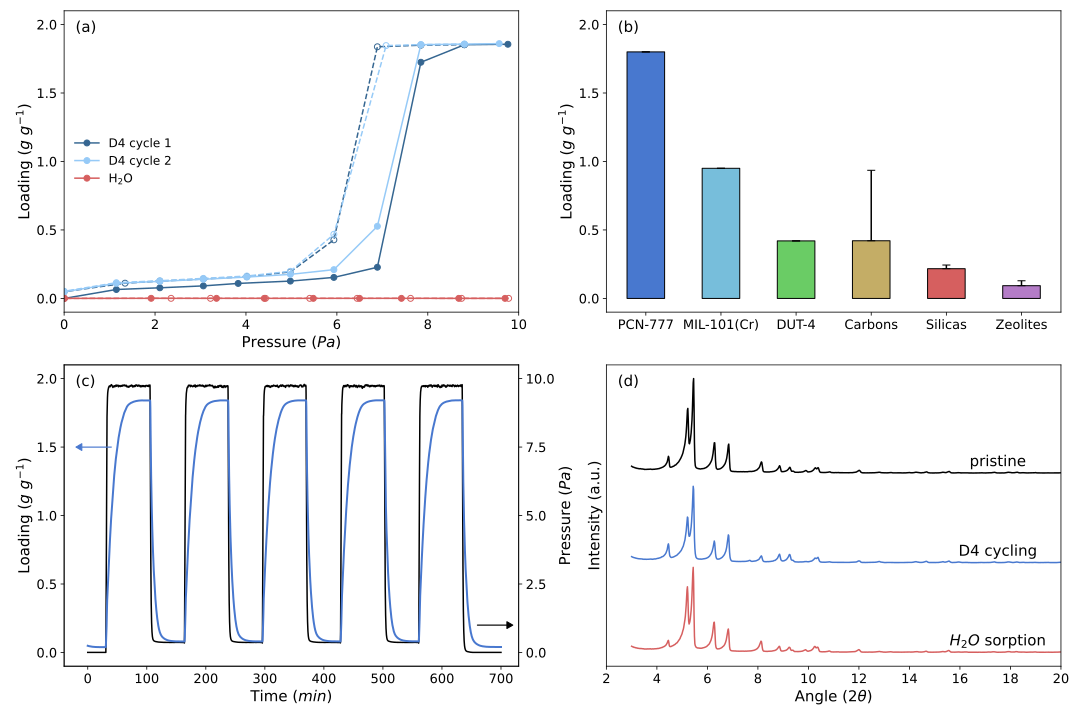
\includegraphics[width=0.95\textwidth]{d4-experiment}
    \caption{%
        (a) Single component adsorption/desorption isotherms for D4 (blue) and
        \ce{H2O} (red) collected at \SI{303}{\kelvin} for PCN-777 in the
        pressure range of 0-\SI{10}{\pascal} (corresponding to 0--0.05
        p/p\textsuperscript{0} for D4). Solid and open symbols represent
        adsorption and desorption branches, respectively. (b) Comparison of the
        D4 capacity of MOFs with other classes of porous materials as detailed
        in Ref \citep{wangRecentAdvancesTechnologies2019}, (c) 5 D4
        sorption-desorption cycles recorded after the first two isotherms on
        PCN-777, in the same pressure range. (d) PXRD of pristine PCN-777
        (black) and samples recovered after D4 cycling (blue) and water
        adsorption (red)
    }\label{fig:d4-experiment}
\end{widefigure}

Throughout desorption (dotted line with open symbols in
\cref{fig:d4-experiment}a), a small hysteresis occurs with a width of about
\SI{1}{\pascal}. Under complete vacuum, a minute amount of D4, about
\SI{0.1}{\gram\per\gram}, i.e. 5\% of total capacity, is retained in the
structure. We attribute this capacity loss to D4 molecules possibly retained in
the super-tetrahedral cages or on a small fraction of defect sites. Overall,
PCN-777 acts as a highly reversible D4-adsorbent. A second sorption cycle
reveals the excellent repeatability of D4 sorption by this MOF, with identical
condensation pressure and total uptake, the adsorption-desorption branches now
overlapping in the very low-pressure region (\cref{fig:d4-experiment}a).

To further investigate the D4 adsorption-desorption cyclability of PCN-777, a
subsequent set of five cycles was recorded on the same sample, covering the
entire uptake range from fully loaded to empty under a medium vacuum level of
\SI{0.5}{\pascal} (see \cref{fig:d4-experiment}b). No further capacity loss is
observed after the initial 5 wt\% from cycle 1 to cycle 2 with a pressure drop
sufficient to fully remove adsorbed D4 in every cycle without the need of
thermal treatment. This is in stark contrast with the previous MOF candidates,
i.e. MIL-101(Cr), and DUT-4. The former was reported
\citep{gargiuloChromiumbasedMIL101Metal2019} to be fully regenerable at only
high temperatures (outgassed under vacuum at \SI{423}{\kelvin}), and we note
that vacuum alone was unable to fully desorb D4, with nearly 50\% of siloxane
remaining in the structure after desorption in our experiments
(\cref{fig:d4-benchmark}, SI). D4 adsorption in DUT-4 is even more irreversible,
owing to the strong confinement of D4 in the pores
\citep{mito-okaSiloxaneD4Capture2013}, with essentially no desorption observed
under vacuum (\cref{fig:d4-benchmark}, SI). The global sorption kinetics was
further qualitatively evaluated by observing the equilibration time throughout
cycling steps. \cref{fig:d4-experiment}b reveals that an adsorption/desorption
cycle can be achieved in less than 30 minutes. Such a fast kinetics is a clear
advantage for practical use. The water adsorption collected for PCN-777 further
confirmed its predicted hydrophobicity and revealed that below
P=\SI{7}{\pascal}, the water loading is negligible, under
\SI{0.02}{\gram\per\gram} (see \cref{fig:d4-experiment}a). This observation
strongly suggests that PCN-777 is expected to maintain its high-level
performance for D4 removal under low to moderate humidity working conditions.

Finally, stability of PCN-777 after its use as a D4 adsorbent has been evaluated
by checking its crystallinity and porosity. PXRD patterns recorded after the D4
cycling experiments show similar Bragg peak positions and broadenings as the
pristine material, testifying that no amorphisation and decrease of
crystallinity was incurred (\cref{fig:d4-experiment}d). The same conclusion
holds true for PCN-777 upon water adsorption. Further, \ce{N2} adsorption
isotherms collected at \SI{77}{\kelvin} for PCN-777 after \ce{H2O} and D4
adsorption both present a similar shape than for the pristine solid (see
\cref{fig:n2-phys}) while slightly lower pore volume
(\SI{1.87}{\centi\metre\cubed\per\gram} vs
\SI{2.20}{\centi\metre\cubed\per\gram}) and BET area
(\SI{1544}{\metre\squared\per\gram} vs \SI{1730}{\metre\squared\per\gram}) were
obtained for the material after D4 cycling, attributed to the small amount of D4
retained in the porous framework during the first adsorption cycle.

\subsection{Adsorption mechanism}\label{adsorption-mechanism}

A careful analysis of the adsorption mechanism of D4 in PCN-777 was further
explored by considering MC simulations in the NVT ensemble with increasing
loading up to the saturation (see methodology section for computational
details). At the initial stage of adsorption, the coordinated OH/\ce{H2O}
moieties of the MOF \ce{Zr6O4} polyhedra pointing towards the pore were found to
act as primary adsorption sites (\cref{fig:d4-mechanistic}a). The D4 molecules
interact mostly via its methyl group with an averaged separating
\ce{H(CH3)-H(H2O)} distance of 2.8 Å (see the radial distribution function
plotted for the corresponding pair in \cref{fig:d4-rdf}a) as illustrated in
\cref{fig:d4-mechanistic}a. This associated preferential sitting of D4 is
associated with a relatively high simulated adsorption enthalpy of
\SI{83.5}{\kilo\joule\per\mol} in line with the isosteric heat of adsorption we
assessed experimentally that ranges from 65 and \SI{75}{\kilo\joule\per\mol}
(\cref{fig:isosteric-enth}), i.e. about \SI{20}{\kilo\joule\per\mol} higher than
the enthalpy of liquefaction of D4 at \SI{303}{\kelvin}
(\SI{54.5}{\kilo\joule\per\mol} \citep{lemmonNISTStandardReference2018}). We
further demonstrated that this value remains substantially lower than the one
simulated for DUT-4 (\SI{194.0}{\kilo\joule\per\mol}) for which the adsorption
of D4 is governed by a high degree of confinement and indeed an irreversible
adsorption. This observation clearly states that the adsorption energetics in
PCN-777 offers a good compromise to ensure an efficient adsorption of D4 as well
as an almost fully reversible and fast adsorption/desorption process. While
increasing the loading, D4 molecules tend to form a monolayer near the wall of
the cage owing to their interactions with both the organic linkers and inorganic
nodes of the MOF as shown in \cref{fig:d4-mechanistic}b-c. Finally, at higher
loading, the molecules occupy the whole cage (\cref{fig:d4-mechanistic}d), the
distribution of the molecules being governed by guest-guest interactions
involving averaged separating \ce{H(CH3)-H(CH3)} distance of 2.7 Å (the radial
distribution function plotted for this pair us shown in \cref{fig:d4-rdf}b) at
the saturation. Such pore filling mechanism has been commonly observed in
mesoporous MOFs for a range of molecules
\citep{zhengMolecularInsightFluorocarbon2020}. Indeed, PCN-777 exhibits an ideal
combination of a large cage to enable an efficient packing of the siloxane
molecules and presence of moieties accessible to D4 to favour host/guest
interactions strong enough to ensure an efficient removal of the first D4
molecules.

\begin{widefigure}[tb]
    \centering
    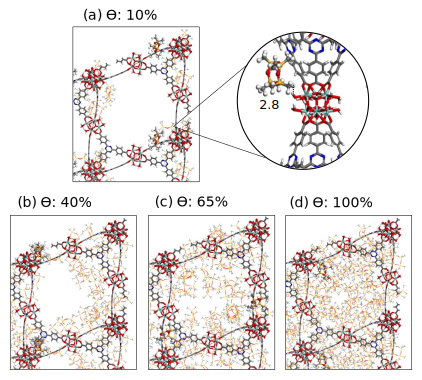
\includegraphics[width=0.9\textwidth]{mechanistic}
    \caption{%
        Representative snapshots of the preferential sitting of D4 for increasing
        loading at (a) 10\% with highlighted interactions distance between D4 and the
        MOF framework, and at (b) 40\%, (c) 65\%, and (d) 100\% fractional loading
        (\(\theta\)) in the pores of PCN-777 at \SI{298}{\kelvin}. Framework atoms
        (sticks) and D4 molecules (lines, and ball and sticks) are coded as Zr, N, O,
        Si, C, and H atoms in light blue, dark blue, red, yellow, dark grey, and light
        grey respectively. The atomic distance is represented by dashed black lines and
        reported in Å.
    }\label{fig:d4-mechanistic}
\end{widefigure}

\section{Conclusion}\label{conclusion}

In this work, a high throughput computational screening first identified a
series of hydrophobic MOFs with octamethylcyclotetrasiloxane uptakes
outperforming by far the performance of the conventional adsorbents. The
best-predicted performer MOF, PCN-777, was synthesized and its predicted
exceptional adsorption capacity for this typical contaminant present in biogas
was further experimentally confirmed. This stable MOF was demonstrated to
exhibit record gravimetric (\SI{1.8}{\gram\per\gram}) and volumetric
(\SI{0.49}{\gram\per\centi\metre\cubed}) uptake alongside with a reversible and fast
adsorption/desorption process, very good cyclability and easy regeneration under
continuous pressure cycling owing to a step-like sorption isotherm. The
attractiveness of PCN-777 was found to result from a synergistic combination of
mesoporous cages and chemical functionality pointing towards the center of the
cages that enables an optimal packing of the siloxane molecule and moderately
high host/guest interactions to favour an efficient removal at low pressure
while maintaining the process highly reversible. Moreover, its hydrophobicity
makes this MOF promising for the selective removal of siloxane molecule in
moderate humidity conditions. In a broader sense, this study highlights the
efficacy of an integrated workflow for accelerating the selection of adsorbents
for a target application, spanning the entire pipeline from method validation to
computational screening, synthesis, adsorption testing and finally
identification of the optimal candidates.

\section{Methodology}\label{methodology}

\subsection{Computational methods}\label{methodology-computational}

The CoRE (Computation-Ready, Experimental) MOF 2019 database
\citep{chungAdvancesUpdatesAnalytics2019} was considered in this work. The
geometric characterization of MOFs, including pore limiting diameters (PLDs),
densities, surface areas (SAs), pore volumes (PVs) and void fractions
(\(\phi\)), were calculated by Zeo++ software
\citep{willemsAlgorithmsToolsHighthroughput2012}. For SA calculations, the
kinetic diameter of nitrogen (\ce{N2}) was used as 3.68 Å and the trial number
was set to 2000. For PV calculations, a zero-probe radius was used, and the
trial number was set to 50 000. We selected 1710 out of 14 000 MOFs, whose PLDs
were large enough to host D4 molecules. 29 well-known MOFs were added in our
dataset for their stability and high porosity. More information about our
dataset can be found in SI.

All Monte Carlo simulations were performed with the RASPA simulation package
\citep{dubbeldamRASPAMolecularSimulation2016}. Henry constants of \ce{H2O} and
isosteric enthalpy of adsorption (\(\Delta H_{st,H_{2}O}^{0}\)) values for all
MOFs were initially computed at \SI{298}{\kelvin} and zero coverage (infinite
dilution) using the Widom particle insertion method
\citep{frenkelUnderstandingMolecularSimulation2002} following the protocol of
Moghadam and coworkers \citep{moghadamEfficientIdentificationHydrophobic2016}
\ce{H2O} molecule was modelled using TIP4P/2005
\citep{abascalGeneralPurposeModel2005} Simulations for \ce{H2O} affinities were
carried out for 1 × 10\textsuperscript{5} Monte Carlo (MC) steps with 5 ×
10\textsuperscript{4} steps for initialization.

D4 was modelled as a semi-flexible molecule with an all atom atomistic model.
All intramolecular bonds, angles, dihedrals, and cross terms parameters for
methyl groups were taken from the consistent-valence force field (CVFF).
\citep{dauber-osguthorpeStructureEnergeticsLigand1988}
(\cref{tbl:ff-d4-bond,tbl:ff-d4-bend,tbl:ff-d4-dihedral,tbl:ff-d4-cross-bond,tbl:ff-d4-cross-bondbend},
SI). All atoms of D4 were treated as Lennard-Jones charged sites. The electronic
potential (ESP) derived partial charges of D4 were computed by density
functional theory (DFT) calculations with PBE (Perdew-Burke-Ernzerhof)
functional \citep{perdewGeneralizedGradientApproximation1996} and DNP (double
numeric plus polarization) basis set
\citep{hehreSelfconsistentMolecularOrbital1972}, using DMol\textsuperscript{3}
module \citep{delleyAllElectronNumerical1990} in Materials Studio
\citep{accelrysMaterialsStudio2001} (\cref{tbl:ff-d4-charge}). Matsubara and
coworkers \citep{matsubaraDesignVersatileForce2010} developed a force field for
the molecular simulation of D4 molecules which methyl groups were modelled as a
single-site. Whereas this model was useful to understand the atomic scale of D4,
we developed a novel model including all atoms in D4 in this study. The LJ
\(\epsilon\) (K) and \(\sigma\) (Å) parameters for all atoms of D4 were then
taken from the universal force field (UFF) \citep{rappeUFFFullPeriodic1992}.
Atomic charges of all atoms in the MOFs were estimated using Extended Charge
Equilibration (Qeq) method as implemented in RASPA
\citep{dubbeldamRASPAMolecularSimulation2016} and their LJ parameters were taken
from the UFF forcefield as currently employed
\citep{qiaoHighthroughputComputationalScreening2017,
keskinProgressOpportunitiesChallenges2009}. Continuous fractional component
Monte Carlo (CFCMC) simulations were performed to estimate saturation uptake of
D4 in MOFs at \SI{298}{\kelvin}. All CFCMC simulations were carried out for a
total of 1 × 10\textsuperscript{4} steps with the first 5 ×
10\textsuperscript{3} steps for equilibration and the last 5 ×
10\textsuperscript{3} steps for production. A step consists of N Monte Carlo
steps; where N is equal to the number of molecules (which fluctuates during a
CFCMC simulation). All simulations included random insertion, rotation,
translation and continuous-fractional swap lambda moves with an equal
probability. The D4/MOF interactions were described by the sum of van der Waals
(LJ) and Coulombic terms. The electrostatic interactions were calculated by the
Ewald summation \citep{ewaldBerechnungOptischerUnd1921} while a cut-off radius
of 12.8 Å was considered for the van-der-Waals term. Cell lengths of the
simulations were increased to at least 25.6 Å in each three dimensions and all
MOF frameworks were considered as rigid in the simulations.

The geometry optimization of PCN-777 at the density-functional theory (DFT)
level was performed using the CP2K package
\cite{vandevondeleQuickstepFastAccurate2005} using PBE functional
\citep{perdewGeneralizedGradientApproximation1996} with GTH
(Goedecker-Teter-Hutter) pseudopotentials
\citep{goedeckerSeparableDualspaceGaussian1996}, the TZV2P-MOLOPT-GTH for H, C,
N, and O atoms and DZVP-MOLOPT-SR-GTH for Zr atoms. The auxiliary plane-wave
basis sets were truncated at 400 Ry. The unit cell parameters and all atomic
positions in the framework were fully relaxed in this simulation. The restrained
electrostatic potential (RESP) charges for these atoms of the framework were
calculated with CP2K package using PBE functional and using similar correlation
functional.

We ran NVT simulations with the loading different number of molecules per unit
cell to understand adsorption mechanism at various fractional uptake. In NVT
simulations, we performed a total 1 × 10\textsuperscript{5} steps with the first
5 × 10\textsuperscript{4} steps for initialization. With the equal probability
of translation, random translation, rotation, and continuous-fractional swap
moves were chosen to identify the model of D4 molecule. MC simulations were
finally performed to investigate Henry’s constant of D4 and isosteric enthalpy
of adsorption for D4 in three MOFs including PCN-777, DUT-5 and MIL-101 at
infinite dilution and \SI{298}{\kelvin} by using Widom particle insertion method
\citep{frenkelUnderstandingMolecularSimulation2002}. For each material, MC
simulations were carried out for a total 1 × 10\textsuperscript{6} steps with
the first 5 × 10\textsuperscript{5} steps for initialization. It should be also
noted that D4 molecule was modelled fully rigid while the same LJ 12--6
forcefields were used (\cref{tbl:ff-d4-charge}).

\subsection{Dataset}

All the results of the HCTS are available in as CSV files in the SI. An
web-based explorer, which can be used to interactively display the dataset is
available at \url{https://pauliacomi.com/mof4d4}.

\subsection{D4 sorption experiments}\label{methodology-d4sorption}

Sorption measurements were gravimetrically recorded using a dynamic method in a
DVS Vacuum instrument (Surface Measurement Systems, UK). In this setup, a
continuous adsorbate flow enters the sample enclosure, passes the suspended
sample pan, and is entrained by a vacuum system. Pressure controlled by a
PID-controlled butterfly valve located before the outlet. Probe vapour is
sourced from the headspace of a temperature-controlled reservoir. Uptake is
monitored by a magnetically suspended balance, capable of measuring mass changes
at a resolution of \SI{0.1}{\micro\gram}. The entire sample enclosure is kept in
a temperature-controlled chamber to avoid any condensation points. The D4 used
for the sorption experiments was sourced from Sigma Aldrich, with minimum 98 \%
purity. For each experiment, a stainless-steel sample pan is first tared, then
loaded with about \SI{10}{\milli\gram} of sample. The sample is activated
\emph{in situ} through heating the sample under dynamic vacuum
(\SI{1E-2}{\pascal}) to \SI{423}{\kelvin} (\SI{150}{\degreeCelsius}). The
adsorption-desorption isotherms for D4 and \ce{H2O} and subsequent repeats were
recorded at \SI{303}{\kelvin} (\SI{30}{\degreeCelsius}) in the
0-\SI{10}{\pascal} range of pressure. Adsorption cycling was similarly recorded,
switching between two setpoints of low (\SI{0.5}{\pascal}) and high pressure
(\SI{10}{\pascal}).

\subsection{Benchmark sorbents}\label{methodology-benchmark-sorbents}

The benchmark MIL-101(Cr) sample was taken from a previous work
\citep{pillaiCapturePerformancesHybrid2017}, with all textural characteristics
as stated in reference. DUT-4 was purchased from Materials Center (TU Dresden,
Germany). PXRD, TGA and \ce{N2} physisorption measurements for DUT-4 are
available in the SI (\cref{fig:dut4-summary}). BET surface areas of
\SI{3475}{\metre\squared\per\gram} and \SI{1610}{\metre\squared\per\gram} were
determined for MIL101(Cr) and DUT-4, respectively. Both samples were activated
at \SI{150}{\degreeCelsius} under vacuum before D4 adsorption experiments.

\subsection{PCN-777 synthesis}\label{methodology-pcn777-synthesis}

PCN-777 was synthesised by optimizing a previous published methodology
\citep{fengHighlyStableZeotype2015}. Full synthesis methodology, activation
procedure and phase purity analysis using TGA, PXRD and \ce{N2} physisorption
are given in the SI.

\subsection{Material characterization}\label{methodology-characterization}

PXRD patterns were recorded on a Panalytical X'Pert PRO PXRD diffractometer with
a Cu \(K_{\alpha}\) radiation source, in a Bragg-Brentano reflection geometry,
using a spinning sample holder with a low-background silicon insert. Nitrogen
isotherms at \SI{77}{\kelvin} were recorded in a Micromeritics Tristar
manometric analyser (see SI for detailed methodology). The Brunauer-Emmet-Teller
area was calculated using the pyGAPS suite
\citep{iacomiPyGAPSPythonbasedFramework2019}, with the application of the
Rouquerol rules for isotherm region selection yielding a minimum Pearson
correlation coefficient of r=0.997 (see \cref{fig:n2-analysis} for resulting
fitting).
